\documentclass[dvipsnames,11pt]{article}
\usepackage{amsmath}

%Hey, if you're using this preamble it means that it was probably written by Stefano Graziosi (me). If you see something that doesn't make sense, feel free to email me at stefano.graziosi@studbocconi.it
%p.s. in case it's not already evident from the preamble, I'm not a professional LaTeX user, so I'm sure there are better ways to do things. I'm just trying to make it work.

%------------------------------------------------------------------------------
%           LAST UPDATE: 30-01-2025
%------------------------------------------------------------------------------

%I don't own copyright on anything, I just literally copied and pasted together a bunch of stuff.

%Credit goes to the original authors.

%------------------------------------------------------------------------------
%           Packages
%------------------------------------------------------------------------------

\usepackage{fancyhdr}
\usepackage[dvipsnames]{xcolor}
\usepackage[many]{tcolorbox}
\usepackage[all]{xy}
\usepackage{tcolorbox}
\usepackage{graphicx}
\usepackage{hyperref}
\usepackage{xcolor}    
\usepackage{wrapfig}
\usepackage{amsmath, amssymb, amsthm}
\usepackage{titlesec}
\usepackage{halloweenmath}
\usepackage{enumitem}
\usepackage{listings}
\usepackage{kantlipsum}
\usepackage{pdfpages}

\usepackage[T1]{fontenc}                            % Font Styling
\usepackage{lmodern,mathrsfs}


\usepackage{mathtools,amsthm,amssymb,amsfonts,bm}   % Math Presets
\usepackage{thmtools,amsmath}
\usepackage{array,tabularx,booktabs}                % Table Presets
\usepackage{graphicx,wrapfig,float,caption}         % Figure Presets
\usepackage{setspace,multicol}                      % Text Presets
\usepackage{tikz,physics}                           % Physics Presets

\usepackage{titlepic}
\usepackage{pdfpages}

%------------------------------------------------------------------------------
%           Geometry
%------------------------------------------------------------------------------

\usepackage[a4paper,margin=1in]{geometry}
%\usepackage[margin=1in]{geometry}

%------------------------------------------------------------------------------
%           Chapter and section formatting
%------------------------------------------------------------------------------

%\renewcommand{\chaptername}{Lecture}
%\renewcommand\thesection{P~\arabic{section}}

\renewcommand{\thefigure}{\thesection-\arabic{figure}}
\renewcommand{\thetable}{\thesection-\arabic{table}}

%------------------------------------------------------------------------------
%           Colours
%------------------------------------------------------------------------------

\definecolor{sgblue}{rgb}{0, 169, 211}
\definecolor{sggreen}{rgb}{0, 164, 0}
\definecolor{sgpurple}{rgb}{99, 0, 165}
\definecolor{sgyellow}{rgb}{255, 211, 0}
\definecolor{sgorange}{rgb}{255, 127, 20}

\definecolor{sbblue}{rgb}{219, 248, 254}
\definecolor{sbgreen}{rgb}{223, 255, 218}
\definecolor{sbpurple}{rgb}{241, 220, 255}

\definecolor{codegreen}{rgb}{0,0.6,0}
\definecolor{codegray}{rgb}{0.5,0.5,0.5}
\definecolor{codepurple}{rgb}{0.58,0,0.82}
\definecolor{backcolour}{rgb}{0.95,0.95,0.92}

%------------------------------------------------------------------------------
%           Environments
%------------------------------------------------------------------------------

%Standard \latex box

\newtcolorbox{mybox}[3][]
{
  colframe = #2!25,
  colback  = #2!10,
  coltitle = #2!20!black,  
  title    = {#3},
  #1,
}

%Standard "Problem" environment

\newtheorem{problem}{Problem}

%Personalised "Solution" environment

\newenvironment{solution}[1][\it{\textcolor{MidnightBlue}{Solution}}]{\textbf{#1. } }{\textcolor{MidnightBlue}{$\square$}}


% ----------------------------------------------------------------------
%           Special Environments 
% ----------------------------------------------------------------------

\newlength{\spacelength}
\settowidth{\spacelength}{\normalfont\ }
\declaretheoremstyle[
    headfont={\bfseries\sffamily\footnotesize},
    notefont={\normalfont},
    bodyfont={\normalfont},
    headpunct={\relax},%\newline,
    headformat={%
        \makebox[0pt][r]{\NAME\ \NUMBER\hspace{\marginparsep}}\hskip-\spacelength{\normalsize\NOTE}},
]{theorem}

\tcolorboxenvironment{theorem}{
  boxrule=0pt,
  boxsep=0pt,
  colback={White},
  enhanced jigsaw, 
  borderline west={1pt}{0pt}{ForestGreen},
  sharp corners,
  before skip=10pt,
  after skip=10pt,
  left=5pt,
  right=5pt,
  breakable,
}

\declaretheorem[style=theorem]{proposition}

\let\proof\relax
\let\endproof\relax

\declaretheoremstyle[
    headfont={\bfseries\sffamily\footnotesize},
    notefont={\normalfont},
    bodyfont={\normalfont},
    headpunct={\relax},%\newline,
    headformat={%
        \makebox[0pt][r]{\NAME\ \NUMBER\hspace{\marginparsep}}\hskip-\spacelength{\normalsize\NOTE}},
]{theorem}

\tcolorboxenvironment{proposition}{
  boxrule=0pt,
  boxsep=0pt,
  colback={White},
  enhanced jigsaw, 
  borderline west={1pt}{0pt}{Mulberry},
  sharp corners,
  before skip=10pt,
  after skip=10pt,
  left=5pt,
  right=5pt,
  breakable,
}

\declaretheorem[style=theorem]{theorem}

\let\proof\relax
\let\endproof\relax

\declaretheoremstyle[
    headfont={\small\scshape},
    notefont={\normalfont},
    bodyfont={\normalfont},
    headpunct={\relax},
    headformat={%
        \makebox[0pt][r]{\NAME\hspace{\marginparsep}}\hskip-\spacelength{\NOTE}},
]{proof}

\tcolorboxenvironment{proof}{
  boxrule=0pt,
  boxsep=0pt,
  blanker,
  borderline west={1pt}{0pt}{black},
  before skip=10pt,
  after skip=10pt,
  left=5pt,
  right=5pt,
  breakable,
}

\declaretheoremstyle[
    headfont={\footnotesize\itshape},
    notefont={\normalfont},
    bodyfont={\normalfont},
    headpunct={\relax},
    headformat={%
        \makebox[0pt][r]{\NAME\hspace{\marginparsep}}\hskip-\spacelength{\NOTE}},
]{claim}

\declaretheorem[
    style=proof,
    qed=\qedsymbol]{proof}

\declaretheorem[style=claim]{Intuition}

\theoremstyle{theorem}
\newtheorem{ques}{Question}

\theoremstyle{theorem}
\newtheorem{definition}{Definition}
\tcolorboxenvironment{definition}{
  boxrule=0pt,
  boxsep=0pt,
  colback={White},
  enhanced jigsaw, 
  borderline west={1pt}{0pt}{Cerulean},
  sharp corners,
  before skip=10pt,
  after skip=10pt,
  left=5pt,
  right=5pt,
  breakable,
}

\theoremstyle{theorem}
\newtheorem{lemma}{Lemma}
\tcolorboxenvironment{lemma}{
  boxrule=0pt,
  boxsep=0pt,
  blanker,
  borderline west={1pt}{0pt}{Rhodamine},
  before skip=10pt,
  after skip=10pt,
  sharp corners,
  left=5pt,
  right=5pt,
  breakable,
}

\theoremstyle{theorem}
\newtheorem{remark}{Remark}
\tcolorboxenvironment{remark}{
  boxrule=0pt,
  boxsep=0pt,
  colback={White},
  enhanced jigsaw, 
  borderline west={1pt}{0pt}{BurntOrange},
  before skip=10pt,
  after skip=10pt,
  sharp corners,
  left=5pt,
  right=5pt,
  breakable,
}

\theoremstyle{theorem}
\newtheorem{corollary}{Corollary}
\tcolorboxenvironment{corollary}{
  boxrule=0pt,
  boxsep=0pt,
%  colback={White!100!WildStrawberry},
  enhanced jigsaw,
  borderline west={1pt}{0pt}{WildStrawberry},
  before skip=10pt,
  after skip=10pt,
  sharp corners,
  left=5pt,
  right=5pt,
  breakable,
}

\theoremstyle{theorem}
\newtheorem{example}{Example}
\tcolorboxenvironment{example}{
  boxrule=0pt,
  boxsep=0pt,
  blanker,
  borderline west={1pt}{0pt}{Dandelion},
  before skip=10pt,
  after skip=10pt,
  sharp corners,
  left=5pt,
  right=5pt,
  breakable,
}


\theoremstyle{claim}
\newtheorem{intu}{Intuition}

\theoremstyle{claim}
\newtheorem{solu}{Solution}

%------------------------------------------------------------------------------
%           Code Listing Environment
%------------------------------------------------------------------------------

\lstdefinestyle{mystyle}{
    backgroundcolor=\color{backcolour},   
    commentstyle=\color{codegreen},
    keywordstyle=\color{magenta},
    numberstyle=\tiny\color{codegray},
    stringstyle=\color{codepurple},
    basicstyle=\ttfamily\footnotesize,
    breakatwhitespace=false,         
    breaklines=true,                 
    captionpos=b,                    
    keepspaces=true,                 
    numbers=left,                    
    numbersep=5pt,                  
    showspaces=false,                
    showstringspaces=false,
    showtabs=false,                  
    tabsize=2
}

\lstset{style=mystyle}

\setlength{\headheight}{25pt} % Non so perché ma senza questo da un piccolo errore

\pagestyle{fancy}
\fancyhf{} 
\fancyhead[L]{\textsc{\footnotesize{PhD in Economics and Finance} \\ \small{40313 Introd. to Probability}}} 
\fancyhead[R]{\textsc{\small Graziosi \\ Natalucci}} 
\fancyhead[C]{\textbf{Problem set 4}}
\fancyfoot[C]{\thepage} 
\renewcommand{\headrulewidth}{0.4pt} 
\renewcommand{\footrulewidth}{0pt}

\begin{document}

\section*{Question 1}

    Let $Z$ be a random variable with uniform distribution on $(0,1)$ and let $X_1,X_2$ be conditionally independent and identically distributed, given $Z$ with $P(X_i=1|Z)=1-P(X_i=0|Z)=Z$ ($i=1,2$).

    \begin{enumerate}[label=\alph*.]
        \item Find $E(X_i )$ and $V (X_i )$ ($i=1,2$).
    
            \begin{solution}
    
                By the law of total expectation, $E(X_i)=E\big(E(X_i\mid Z)\big)=E(Z)$.
                
                Since $Z\sim \mathrm{Unif}(0,1)$, $E(Z)=\int_0^1 z\,dz=\tfrac12$, hence
                \[
                E(X_i)=\frac12.
                \]
                
                For the variance, we use the variance decomposition (i.e.\ law of total variance):
                \[
                V(X_i)=E\!\big[V(X_i\mid Z)\big]+V\!\big(E(X_i\mid Z)\big)
                =E\!\big[Z(1-Z)\big]+V(Z).
                \]
                
                Now $E[Z(1-Z)]=E(Z)-E(Z^2)=\tfrac12-\tfrac13=\tfrac16$, and
                $V(Z)=E(Z^2)-E(Z)^2=\tfrac13-\tfrac14=\tfrac1{12}$. 
                
                Therefore
                \[
                V(X_i)=\frac16+\frac1{12}=\frac14.
                \]                
                
            \end{solution}
            
        \item Find $Cov(X_1 , X_2 )$.
    
            \begin{solution}
    
                Conditional on $Z$, $X_1$ and $X_2$ are independent, so
                \[
                E(X_1X_2)=E\!\big(E(X_1X_2\mid Z)\big)=E\!\big(E(X_1\mid Z)E(X_2\mid Z)\big)=E(Z^2)=\frac13.
                \]
                
                Thus
                \[
                \mathrm{Cov}(X_1,X_2)=E(X_1X_2)-E(X_1)E(X_2)=\frac13-\frac12\cdot\frac12=\frac13-\frac14=\frac1{12}.
                \]
                
            \end{solution}
            
        \item Are $X_1,X_2$ stochastically independent?
    
            \begin{solution}
    
                \textbf{No}. Independence would require $P(X_1=1,X_2=1)=P(X_1=1)P(X_2=1)$. 
                
                But
                \[
                P(X_1=1,X_2=1)=E(Z^2)=\frac13\neq \left(E(Z)\right)^2=\left(\frac12\right)^2=\frac14.
                \]
                Hence they are not independent (they are exchangeable with positive covariance).
                
            \end{solution}
            
        \item Find $P(Z\leq 1/2\mid X_1=1)$.
    
            \begin{solution}
    
                By Bayes’ rule with a continuous prior (the \emph{Bayesian scheme}), the posterior of $Z$ after one success is
                \[
                Z\mid X_1=1\sim \mathrm{Beta}(1+1,1+0)=\mathrm{Beta}(2,1),
                \]
                with density $f(z\mid X_1=1)=2z\,\mathbf 1_{(0,1)}(z)$. 
                
                Therefore
                \[
                P\big(Z\le \tfrac12 \mid X_1=1\big)=\int_0^{1/2} 2z\,dz=\left.z^2\right|_{0}^{1/2}=\frac14.
                \]

            \end{solution}
            
    \end{enumerate}

%%%%%%%%%%%%%%%%%%%%%%%%%%%%%%%%%%%%%%%%%%%%

\section*{Question 2}

    \begin{enumerate}
        \item Generate in Python 1000 observations $(x_i,y_i)$ from a bivariate normal distribution with mean vector $(0,0)$ and variance-covariance matrix
            \[
            \left[
            \begin{array}{cc}
            1&0.2\\
            0.2&1
            \end{array}
            \right].
            \]

            \begin{solution}

\begin{lstlisting}[language=python]
import numpy as np

# Reproducibility
rng = np.random.default_rng(40313)

# Mean vector and covariance matrix
mu = np.array([0.0, 0.0])
Sigma = np.array([[1.0, 0.2],
                  [0.2, 1.0]])

# Draw 1000 observations
data = rng.multivariate_normal(mean=mu, cov=Sigma, size=1000)
x = data[:, 0]
y = data[:, 1]
\end{lstlisting}
            
            \end{solution}
        
        \item Draw an histogram of $x_1,\dots,x_{1000}$.

            \begin{solution}
    
\begin{lstlisting}[language=python]
import matplotlib.pyplot as plt

fig, ax = plt.subplots()
ax.hist(
    x,
    bins="fd",
    density=True,
    alpha=0.7,
    edgecolor="black",
    linewidth=0.6,
)

ax.set_title("Histogram of x")
ax.set_xlabel("value")
ax.set_ylabel("density")
ax.grid(True, alpha=0.3, linestyle="--", linewidth=0.5)
for spine in ("top", "right"):
    ax.spines[spine].set_visible(False)
fig.tight_layout()
plt.show()

\end{lstlisting}

                \begin{figure}[h]
                    \centering
                    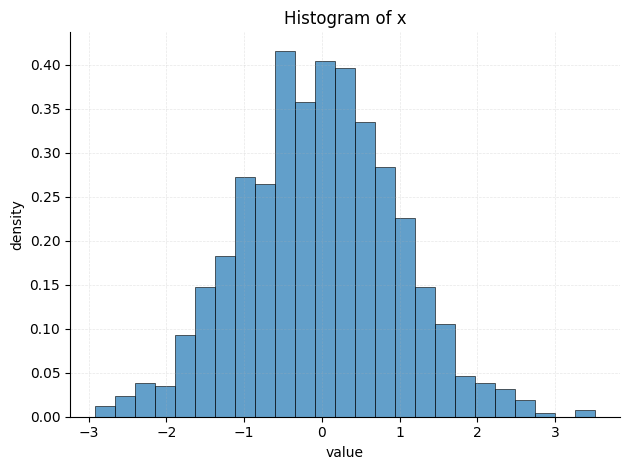
\includegraphics[width=0.5\linewidth]{q2b.png}
                \end{figure}
                
            \end{solution}
            
        \item Draw an histogram of those $y_i$ such that $x_i\leq 0$.

            \begin{solution}
    
\begin{lstlisting}[language=python]
import matplotlib.pyplot as plt
import numpy as np

mask = x <= 0
y_subset = y[mask]

fig, ax = plt.subplots()
ax.hist(
    y_subset,
    bins="fd",
    density=True,
    alpha=0.7,
    edgecolor="black",
    linewidth=0.6,
)

ax.set_title("Histogram of y given x \leq 0")
ax.set_xlabel("value")
ax.set_ylabel("density")
ax.grid(True, alpha=0.3, linestyle="--", linewidth=0.5)
for spine in ("top", "right"):
    ax.spines[spine].set_visible(False)
fig.tight_layout()
plt.show()
\end{lstlisting}
                
                \begin{figure}[h]
                    \centering
                    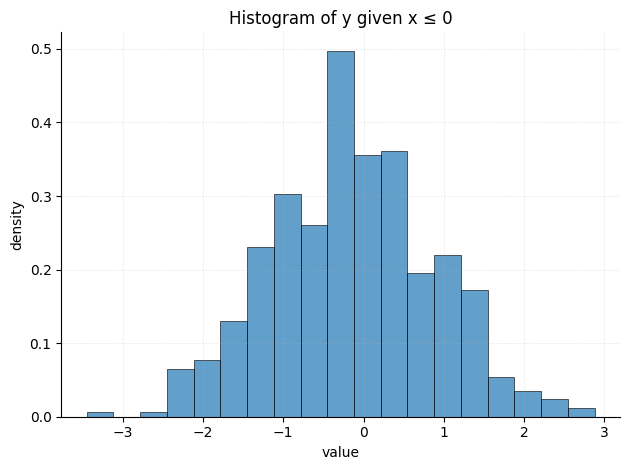
\includegraphics[width=0.5\linewidth]{q2c.png}
                \end{figure}
                
            \end{solution}
            
    \end{enumerate}

\end{document}
